% A quotation in a small-font node, then a frame fitted around it:
% csquotes asks \lastskip and \lastkern while the word is set, and the
% first use of the size writes a font message and sets its expansion.
\documentclass{article}
\usepackage{newtxtext}
\usepackage[T1]{fontenc}
\usepackage{csquotes}
\usepackage{microtype}
\usepackage{tikz}
\usetikzlibrary{fit}
\begin{document}
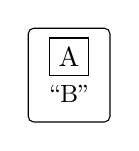
\begin{tikzpicture}
\node[draw] (a) at (0,0) {A};
\node[below,font=\small] (b) at (a.south) {\enquote{B}};
\node[draw,rounded corners=2pt,fit={(a)(b)}] {};
\end{tikzpicture}
\gdef\SatexReachedEnd{}
\end{document}
